\chapter{Background and Related Work}\label{chap.background}
\minitoc

\section{Introduction}

\section{Neural Networks}

\subsection{Convolutional Neural Networks}
\subsubsection{Conv2D Tensor Operation}
A convolutional layer aims to learn and extract feature representations from an input. Each unit of a feature map is connected to a region of neighboring units on the input maps (from the previous layer). This neighborhood in the previous layer is known as the receptive field of such unit. A new feature map can be obtained by first convolving the input maps with a learned kernel and then applying a nonlinear elementwise activation function to the convolved results. All spatial locations on the input maps share a kernel to generate a feature map. All feature maps are obtained by convolving several different kernels~\cite{gu2018recent}.


The 2D convolution process is performed by the \emph{Conv2D} tensor operation, described in \Equ{eq:conv2D}, where $h$ is the input tensor containing the feature maps, $W$ is the convolution kernels (known as filters), and $b$ is the bias vector for the output feature maps~\cite{goodfellow2016deep}. $K\times L\times M$ is the receptive field size, $K\times L$ is the convolution kernel, and $M$ is the number of input channels/feature maps. In this work, the \emph{Conv} is denoted as \emph{Conv2D} operator.
\begin{eqnarray} \label{eq:conv2D}
Conv\left(W,h\right)_{i,j,o}=\sum_{k,l,m}^{K,L,M} h_{(i+k,j+l,m)} W_{(o,k,l,m)}+b_{o}
\end{eqnarray}


\subsection{Spike-by-Spike Neural Networks} 

\label{sec:sbs}

Technically, \gls{sbs} is a spiking neural network based on a
generative probabilistic model. It iteratively finds an estimate of
its input probability distribution $p(s)$ (i.e. the probability of
input node $s$ to stochastically send a spike) by its latent variables
via $r(s) = \sum_i h(i) W(s|i)$, 
where $\vec{h}$ is an inference
population composed of a group of neurons that compete with each
other. An \gls{ip_sbs} sees only the spikes $s_t$ (i.e. the
index identifying the input neuron $s$ which generated that spike at
time $t$ produced by its input neurons, not the underlying input
probability distribution $p(s)$ itself. By counting the spikes
arriving at a group of \gls{sbs} neurons, $p(s)$ is estimated by
$\hat{p}(s) = 1/T \sum_t \delta_{s,s^t}$ after $T$ spikes have been
observed in total. The goal is to generate an internal representation
$r(s)$ from the string of incoming spikes $s_t$ such that the negative
logarithm of the likelihood
$L = C - \sum_\mu \sum_s \hat{p}_\mu(s) log\left( r_\mu(s) \right)$ is
minimized. $C$ is a constant which is independent of the internal
representation $r_\mu(s)$ and $\mu$ denotes one input pattern from an
ensemble of input patterns. Applying a multiplicative gradient descent
method on $L$, an algorithm for iteratively updating $h_\mu(i)$ with
every observed input spike $s_t$ could be derived
\cite{ernst2007efficient}:
\begin{eqnarray} \label{eq:sbs_update}
h_\mu^{new}(i) = \frac{1}{1+\epsilon} \left(h_\mu(i) + \epsilon \frac{h_\mu(i) W(s_t|i) }{\sum_j h_\mu(j) W(s_t|j)} \right) 
\end{eqnarray}
where $\epsilon$ is a parameter that also controls the strength of sparseness of the distribution of latent variables $h_\mu(i)$. Furthermore, $L$ can also be used to derive online and batch learning rules for optimizing the weights $W(s|i)$. The interested reader is referred to \cite{ernst2007efficient} for a more detailed exposition.

From a practical point of view, \gls{sbs} provides a mechanism to obtain a sparse representation of input patterns. Given a set of
training samples $\{x_\eta\}$, it learns weights ($W$), that allow
to express the input patterns as a linear sparse non-negative combination
of features.  During inference, it provides a mechanism for expressing
each test input $x_\mu$ as $x_\mu \approx W\, h_\mu$ where all
entries are non-negative.

The inference procedure consists in generating indices $s_t$
distributed according to a categorical distribution of the input pattern
$s_t \sim \mathrm{Categorical}(x_{\mu}(0), x_{\mu}(1), ..,
x_{\mu}(N-1))$. Starting with a random $h$ and executing
iteratively \Equ{eq:sbs_update} the \gls{sbs} algorithms finds
$h_{\mu}$. The fundamental concept of \gls{sbs} can be extended from vector to matrix
inputs. In this case, the linear operation $W\, h_\mu$ can be replaced by a
convolution to obtain a convolutional \gls{sbs} layer. A detailed description of the \gls{sbs} algorithm is presented in the Appendix~\ref{chap.append}

\subsubsection{Basic Network Overview}

\gls{sbs} network models can be constructed in sequential layered structures \cite{rotermund2019Backpropagation}. Each layer consists of many \glspl{ip_sbs} (represented by $\vec{h}$), while the communication between them is organized by a low bandwidth signal -- the spikes.

The \gls{sbs} layer update is summarized in Algorithm~\ref{alg:sbs}. This is an iterative algorithm, where the number of spikes are denoted as ($N_{Spk}$), which is the number of iterations. As a generative model, each iteration updates the internal representation ($H$) based on the input spikes ($S^{in}_t$). A basic \gls{sbs} network architecture for handwritten digit classification (MNIST) is shown in \fig{fig:sbs_network} and \Tab{tab:sbs_network}. Each \gls{ip_sbs} is an independent computational entity, this allows to design specialized hardware architectures that can be massively parallelized (see \fig{fig:SbS_layer}).


\begin{algorithm}[b!]
	\caption{SbS layer update.}\label{alg:sbs}
	
	\begin{algorithmic}[1]
		\FOR {$t \leftarrow 0$ \textbf{to} $N_{Spk}-1$}
		\FOR {$x \leftarrow 0, y \leftarrow 0$ \textbf{to} $N_X-1, N_Y - 1$}
		\STATE $S^{out}_t(x, y) \sim Categorical( H^{}(x, y, :) ) $
		\FOR {$\Delta_X \leftarrow 0, \Delta_Y \leftarrow 0$ \textbf{to} $K_X - 1,K_Y - 1$}
		\STATE $spk \leftarrow S^{in}_t(x + \Delta_X , y + \Delta_Y)$
		\FOR {$i \leftarrow 0$ \textbf{to} $N_H-1$}
		\STATE $\Delta h(i)
		\leftarrow H^{}(x, y,  i) \cdot W^{}(\Delta_X, \Delta_Y, spk, i)$
		\STATE $r \leftarrow r + \Delta h(i)$
		\ENDFOR
		
		\FOR {$i \leftarrow 0$ \textbf{to} $N_H-1$}
		\STATE $H^{new}(x, y, i) \leftarrow \frac{1}{1+\epsilon} \left( H^{}(x, y, i) + \frac{\epsilon}{r} \Delta h(i) \right) $              
		\ENDFOR
		\ENDFOR
		\ENDFOR
		\ENDFOR
	\end{algorithmic} 
\end{algorithm}

\begin{figure*}[b!]
	\centering
	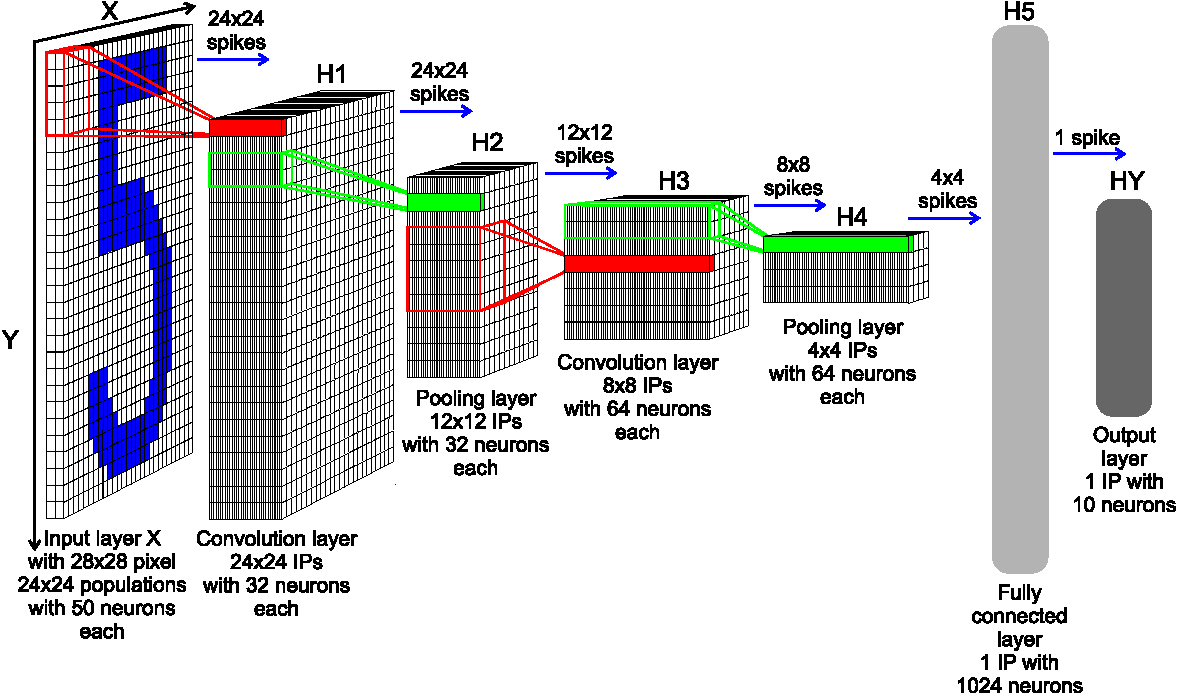
\includegraphics[width=0.5\columnwidth]{./chapters/sbs_accelerator/figures/sbs_network.pdf}
	\caption{\gls{sbs} network architecture for handwritten digit classification task.}
	\label{fig:sbs_network}
\end{figure*}


\begin{table}[t!]\centering
	\caption{\gls{sbs} network architecture for handwritten digit classification task.}
	\label{tab:sbs_network}
	\scriptsize
	\begin{tabular}{lrrrrrrr}\toprule
		&\multicolumn{3}{c}{\textbf{Layer size}} & &\multicolumn{2}{c}{\textbf{Kernel size}} \\\cmidrule{2-4}\cmidrule{6-7}
		\textbf{Layer} ($H^l$) &$N_X$ &$N_Y$ &$N_H$ & &$K_X$ &$K_Y$ \\\midrule
		Input ($HX$) &28 &28 &2 & &- &- \\
		Convolution ($H1$) &24 &24 &32 & &5 &5 \\
		Pooling ($H2$) &12 &12 &32 & &2 &2 \\
		Convolution ($H3$) &8 &8 &64 & &5 &5 \\
		Pooling ($H4$) &4 &4 &64 & &2 &2 \\
		Fully connected ($H5$) &1 &1 &1024 & &4 &4 \\
		Output ($HY$) &1 &1 &10 & &1 &1 \\
		\bottomrule
	\end{tabular}
\end{table}

\subsubsection{Computational Cost}

The number of \gls{mac} operations required for inference of an \gls{sbs} layer is defined by $NOPS_{MAC}=N_{Spk} N_X N_Y K_X K_Y (3 N_H + 2)$, where $N_{Spk}$ is the number of spikes (iterations), $N_X N_Y$ is the size of the layer, $K_X K_Y$ is the size of the kernel for convolution/pooling, and $N_H$ is the length of $\vec{h}$. The computational cost of \gls{sbs} network models is higher compared to equivalent \gls{cnn} models and lower compared to regular \gls{snn} models (e.g., \gls{lif}) \mbox{\cite{izhikevich2004model}}.


\begin{figure*}[b!]
	\centering
	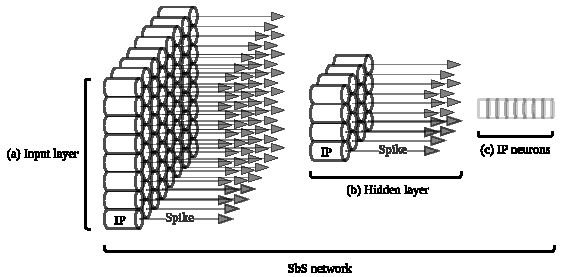
\includegraphics[width=0.5\columnwidth]{./chapters/sbs_accelerator/figures/SbS_layer.pdf}
	\caption{\gls{sbs} \glspl{ip_sbs} as independent computational entities, (a) illustrates an input layer with a massive amount of \glspl{ip_sbs} operating as independent computational entities, (b) shows a hidden layer with an arbitrary amount of \glspl{ip_sbs} as independent computational entities, (c) exhibits a set of neurons grouped in an \gls{ip_sbs}.}
	\label{fig:SbS_layer}
\end{figure*}


\subsubsection{Error Tolerance}

To illustrate the error tolerance of \gls{sbs} networks, it is presented a classification performance under positive additive uniformly distributed noise as external disturbance. \fig{fig:robustnes_sbs} presents a comparison of the classification performance of an \gls{sbs} network and a standard \gls{cnn}, with the same amount of
neurons per layer as well as the same layer structure. Both neural networks are trained for handwritten digit classification on MNIST dataset \cite{lecun1998mnist} (see \cite{rotermund2019Backpropagation} for details). The figure shows the correctness for the MNIST test set with its \num[group-separator={,}]{10000} patterns in dependency of the noise level for positive additive
uniformly distributed noise. The blue curve shows the performance for
the \gls{cnn}, while the red curve shows the performance for
the \gls{sbs} network with \num[group-separator={,}]{1200} spikes (iterations). Beginning
with a noise level of 0.1, the respective performances are different
with a p - level of at least $10^{-6}$ (tested with the Fisher exact
test). Increasing the number of spikes per \gls{sbs} population to \num[group-separator={,}]{6000}
(performance values shown as black stars), shows that more spikes can
improve the performance under noise even more.

\begin{figure*}[b!]
	\centering
	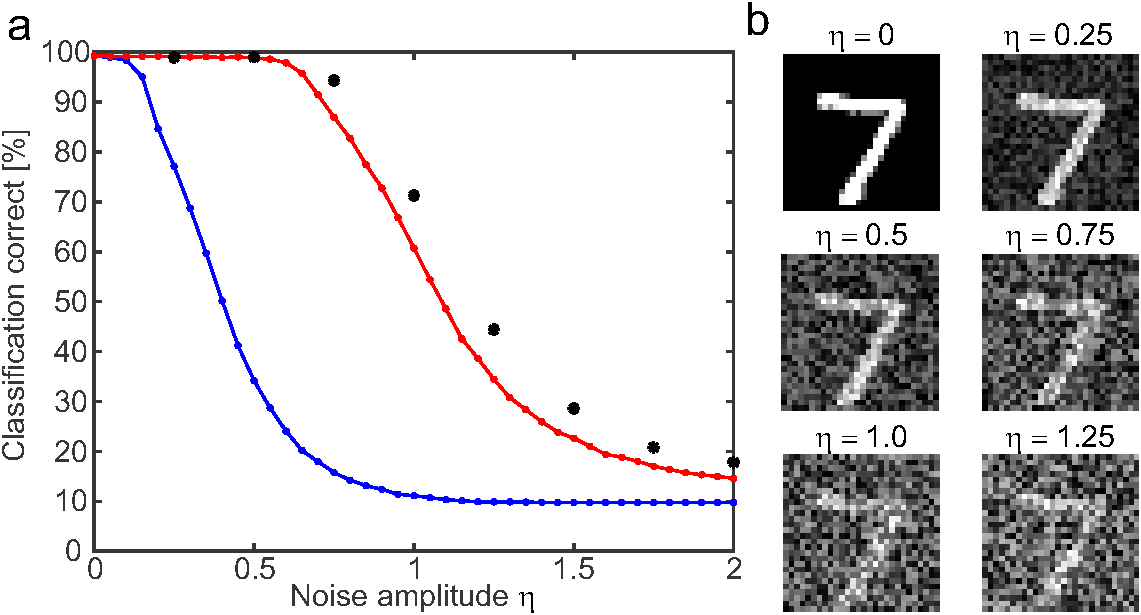
\includegraphics[width=0.5\columnwidth]{./chapters/sbs_accelerator/figures/sbs_robustnes.pdf}
	\caption{(a) Performance classification of \gls{sbs} NN versus equivalent \gls{cnn}, and (b) example of the first pattern in the MNIST test data set with different amounts of positive additive uniformly distributed noise.}
	\label{fig:robustnes_sbs}
\end{figure*}


\section{Neural Network Accelerators}
\subsection{\gls{fpga} Design}
\subsection{Energy-Efficient Dataflow}
\subsection{Reduced Precision}
\subsection{Fixed-Point}
\subsection{Floating-point Number Representation}
The representation of every numerical value, in any numerical system, is made of an integer and a fractional part. The border that delimits them is called the radix point. The fixed-point format for representing numeric values derives its name from the fact that in this format, the base point is fixed at a certain position. For integer numbers, this position is at the right of the least significant digit.

In scientific computation, it is often necessary to represent very large and very small values. This is difficult to achieve using the fixed-point format because the bit size required to maintain both the desired precision and the desired range are very large. In such situations, \gls{fp} formats are used to represent real numbers. Each \gls{fp} number can be divided into three fields: sign $S$, exponent $E$, and mantissa $M$. Using the binary number system, it is possible to represent any \gls{fp} number as:

\begin{eqnarray} \label{eq:float}
(-1)^{S} \times 1.M \times 2^{E-B}
\end{eqnarray}

In \gls{fp} representations the exponent is biased. This bias depends on the bit size of the exponent field. This exponent bias is defined by \Equ{eq:float_bias}, where $E_{size}$ is the exponent bit size.

\begin{eqnarray} \label{eq:float_bias}
B=2^{E_{size}-1}-1
\end{eqnarray}

There is a natural trade-off between small bit size requiring fewer hardware resources and larger bit size providing higher precision. Within a given total bit size, it is possible to assign various combinations of sizes to the exponent and mantissa fields, with wider exponents resulting in a higher range and wider mantissa resulting in better precision.

The most widely used format for \gls{fp} arithmetic is the IEEE 754 standard \cite{zuras2008ieee}. The IEEE single-precision format (32-bit) is expressed by \Equ{eq:float} with $B$ = 127, 8 bits for the exponent and 23 bits for the mantissa, see \Fig{fig:floating}(a). In \gls{fp} formats, the numbers are normalized, the leading one is an implicit bit, and only the fractional part is explicitly stored in the mantissa field.

\begin{figure*}
	\centering
	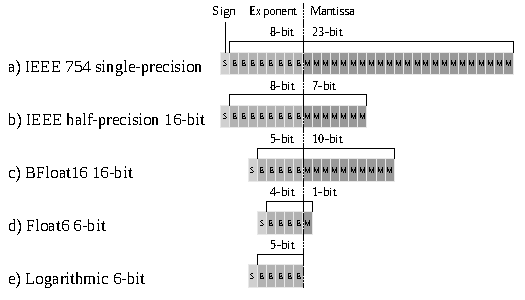
\includegraphics[width=0.5\columnwidth]{./chapters/cnn_accelerator/figures/power_breakdown/floating_point.pdf}
	\caption{Floating-point number representation.}
	\label{fig:floating}
\end{figure*}

Reduced bit size than those specified in the IEEE 754 standard are often sufficient to provide the desired precision. Reduced designs require fewer hardware resources enabling low-power implementations. In custom hardware designs, it is possible to customize the \gls{fp} format implemented. In later sections, the term E$a$M$b$ is used to denote \gls{fp} formats, where $a$ and $b$ are the exponent and mantissa bit size, respectively. For example, E4M1 means 4-bit exponent and 1-bit mantissa, see \Fig{fig:floating}(d).

There are three special definitions in IEEE 754 standard. The first is subnormal numbers when $E=0$, then \Equ{eq:float} is modified to \Equ{eq:float_subnorm}. Infinity and \gls{nan} are the other two special cases but are not used in our work.

\begin{eqnarray} \label{eq:float_subnorm}
(-1)^{S} \times 0.M \times 2^{1-B}
\end{eqnarray}

\section{Related Work}
\subsection{Low-Power Spike-by-Spike Neural Network Accelerators}
For efficient neural network computation, two main optimization strategies are used, namely network compression and classical approximate computing~\cite{bouvier2019spiking}.

\subsubsection{Network Compression}
Researchers focusing on embedded applications started lowering the precision of weights and activation maps to shrink the memory footprint of the large number of parameters representing \glspl{ann}, a method known as network compression or quantization. This practice takes advantage of the intrinsic error-tolerance of neural networks, as well as their ability to compensate for approximation while training. In this way, reduced bit precision causes a small accuracy loss~\cite{courbariaux2015binaryconnect, han2015deep, hubara2017quantized, rastegari2016xnor}.

In hardware development, \gls{wq} has shown up to $2\times$ improvement in energy consumption with an accuracy degradation of less than $1\%$ \cite{moons20160, whatmough201714}. Some advanced quantization methods yield to \glspl{bnn} allowing the use of \glspl{xnor} instead of the conventional costly \glspl{mac}~\cite{rastegari2016xnor}. In~\cite{sun2018xnor}, Sun et al. report an accuracy of $98.43\%$ on handwritten digit classification (MNIST) with a simple \gls{bnn}. Hence, quantization is a powerful tool for improving the energy efficiency and memory requirements of \gls{ann} accelerators, with limited accuracy degradation.

In addition to quantization, network pruning reduces the model size by removing structural portions of the parameters and its associated computations~\cite{lecun1989optimal,hassibi1992second}. This method has been identified as an effective technique to improve the efficiency of \gls{dnn} for applications with limited computational budget~\cite{molchanov2016pruning,li2016pruning, liu2018rethinking}.

These methods can be used for \glspl{snn} as well. In~\cite{rathi2018stdp}, Rathi et al. report up to $3.1\times$ improvement in energy consumption with an accuracy loss of around $3\%$. Weight quantization allows the designer to realize a trade-off between the accuracy of the \gls{snn} application and efficiency of resources. Approximate computing can also be applied at the neuron level, where irrelevant units are deactivated to reduce the computation cost of the \glspl{snn}~\cite{sen2017approximate}. This computation skipping can be applied randomly on synapses, training \glspl{ann} with stochastic synapses improves generalization, resulting in a better accuracy~\cite{srivastava2014dropout, wan2013regularization}. Such methods are compatible with \glspl{snn} and have been tested both during training~\cite{neftci2016stochastic, srinivasan2016magnetic} and operation \cite{buesing2011neural}, and even to define the connectivity between layers \cite{bellec2017deep, chen20184096}. Implementations of spiking neuromorphic systems in \gls{fpga}~\cite{sheik2016synaptic} and hardware~\cite{jerry2017ultra} demonstrated that synaptic stochasticity allows to increase the final accuracy of the networks while reducing memory footprint.

Quantization is therefore a powerful technique to improve energy efficiency and memory requirements of \gls{ann} and \gls{snn} accelerators, with small accuracy degradation. However, this approach requires quantization-aware training methods that, in some cases, are problematic or even inaccessible, particularly in emerging deep \gls{snn} algorithms~\cite{zhang2018survey}.

\subsubsection{Classical Approximate Computing}
Approximate computing has been used in a wide range of applications to increase the computational efficiency in hardware~\cite{han2013approximate}. This approach consists of designing processing elements that approximate their computation by employing modified algorithmic logic units~\cite{han2013approximate}. In~\cite{kim2013energy}, Kim et al. have shown \glspl{snn} using carry skip adders achieving $2.4\times$ latency enhancement and $43\%$ more energy efficiency, with an accuracy degradation of 0.97\% on a handwritten digit classification task (MNIST). Therefore, approximate computing provides important enhancement in energy efficiency and processing speed.

However, as the complexity of the dataset increases, as well as the depth of the network topology, such as ResNet~\cite{he2016deep} on ImageNet~\cite{russakovsky2015imagenet}, the accuracy degradation becomes more important and may not be negligible anymore~\cite{rastegari2016xnor}, especially for critical applications such as autonomous driving. Therefore, it is not certain that network compression techniques and approximate computing are suitable for all applications.

\subsubsection{Spike-by-Spike Neural Network Accelerators}
Rotermund et al. demonstrated the feasibility of a neuromorphic \gls{sbs} \gls{ip_sbs} on a Xilinx Virtex 6 \gls{fpga}~\cite{rotermund2018massively}. It provides a massively parallel architecture, optimized to reduce memory access and suitable for \gls{asic} implementations. Nonetheless, this design is considerably resource-demanding if implemented as a full \gls{sbs} network in today's embedded technology.

\subsection{Low-Power Convolutional Neural Network Accelerators}
\label{sec:related_work}
In the literature we find plenty of hardware architectures for \gls{cnn} accelerators implemented in \gls{fpga}. Most of the research work implements fixed-point quantization, and very limited research focuses on \gls{fp}. Moreover, to the best of my knowledge, there is no research work related to \gls{fp} inference for low-power embedded applications.


\subsubsection{Hybrid Custom Floating-Point}
In \cite{lai2017deep}, Liangzhen Lai et al. proposed a mixed data representation with floating-point for weights and fixed-point for activations. This work demonstrated on SqueezeNet, AlexNet, GoogLeNet, and VGG-16 that 8-bit floating-point quantization (4-bit exponent and 3-bit mantissa) results in constant negligible accuracy degradation. Similarly, in \cite{settle2018quantizing}, Sean O. Settle et al. presented an 8-bit \gls{fp} quantization scheme, which needs an extra inference batch to compensate for quantization errors. However, \cite{lai2017deep} and \cite{settle2018quantizing} did not present a dedicated hardware architecture.

In \cite{lian2019high}, Xiaocong Lian et al. proposed a hardware accelerator with optimized block floating-point (BFP). In this design the activations and weights are represented by 16-bit and 8-bit \gls{fp} formats, respectively. This design is demonstrated on Xilinx VC709 evaluation board. This implementation achieves throughput and power efficiency of \unit[760.83]{GOP/s} and \unit[82.88]{GOP/s/W}, respectively. However, this design is not suitable for low-power resource-constrained embedded \glspl{fpga}.

\subsubsection{Low-Precision Floating-Point}
In \cite{mei2017200mhz}, Chunsheng Mei et al. presented a hardware accelerator for VGG16 model using half-precision \gls{fp} (16-bit). This design is demonstrated on Xilinx Virtex-7 (XC7VX690T) with PCIe interface. This implementation achieves throughput and power efficiency of \unit[202.8]{GFLOP/s} and \unit[18.72]{GFLOP/s/W}, respectively. In \cite{wu2021low}, Chen Wu et al. proposed a low-precision (8-bit) floating-point (LPFP) quantization method for \gls{fpga}-based acceleration. This design is demonstrated on Xilinx Kintex 7 and Ultrascale/Ultrascale+. This implementation achieves throughput and power efficiency of \unit[1086.8]{GOP/s} and \unit[115.4]{GOP/s/W}, respectively.

\subsubsection{Low-Power}
Two research papers have been reported hardware accelerators targeting XC7Z007S. This is the smallest and most inexpensive device from Zynq-7000 SoC family. In \cite{meloni2019cnn}, Paolo Meloni et al. presented a \gls{cnn} inference accelerator for compact and cost-optimized devices. This implementation uses fixed-point to process light-weight \gls{cnn} architectures with a power efficiency between \unit[2.49] to \unit[2.98]{GOPS/s/W}. In \cite{gao2020edgedrnn}, Chang Gao et al. presented EdgeDRNN, a \gls{rnn} accelerator for edge inference. This implementation adopts the \gls{snn} inspired delta network algorithm to exploit temporal sparsity in \glspl{rnn}.
%%%%%%%%%%%%%%%%%%%%%%%%
